\chapter{Recherche}

In diesem Kapitel wird erklärt was BPMN ist, es werden die Rahmenbedingungen umrissen und die verschiedenen Programme analysiert welche für die Umsetzung in Frage kommen.

\section{BPMN}
BPMN steht für Business Process Model and Notation. Dabei handelt es sich um eine genormte Visualisierung für Business Processes. Entwickelt wurde der Standart im Jahre 2001 durch die Firma IBM.

\subsection{Notation}
In diesem Abschnitt soll die grundlegenden Objekte von BPMN vorgestellt werden.

\begin{figure}[H]
	\centering
	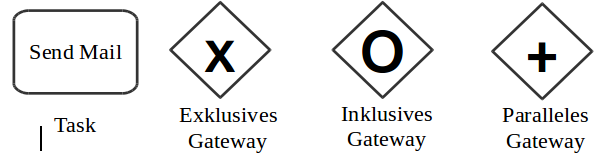
\includegraphics[width=0.6\textwidth]{images/bpmn-flow-objects.png}
	\caption{Flow Objects}
	\label{fig:recherche:bpmn:flowobjects}
\end{figure}
Der Task ist ein Schritt eines Prozesses, welcher ausgeführt wird. Dieser kann entweder durch einen Menschen oder automatisiert durchgeführt werden. Die Rauten sind Gateways. Das Exklusive (XOR) Gateway, steht für einen Entscheidung. Es kann nur ein Pfad weitergeführt werden. Deshalb heisst es exklusiv. Das Inklusive (OR) Gateway ist wie das Exklusive Gateway eine Entscheidung, es können jedoch mehrere Wege parallel ausgeführt werden. Das Paralelle (AND) Gateway führt alle Pfade parallel aus. Es kann auch dazu verwendet werden mehrere Pfade zu synchronisieren und als einzelner Weg weiterzuführen.

\begin{figure}[H]
	\centering
	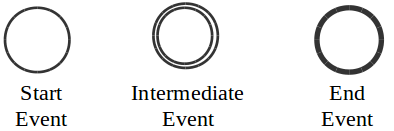
\includegraphics[width=0.4\textwidth]{images/bpmn-flow-objects2.png}
	\caption{Events}
	\label{fig:recherche:bpmn:events}
\end{figure}
Ein Event beschreibt, wenn etwas während eines Prozesses passiert. Oben aufgeführt sind die drei Grundevents. Der Start Event kennzeichnet der Beginn und der End Event das Ende eines Prozesses. Ein Intermediate Event kann irgendwo zwischen dem Start und dem Ende eines Prozesses stehen. Es gibt diverse Ausprägungen von Events, welche mit Icons in den Kreisen gekennzeichnet werden. Zum Beispiel ein Mail Event, Timer Event, Error Event, Cancel Event, Link Event, Signal Event und Terminate Event, um einige zu nennen.

\begin{figure}[H]
	\centering
	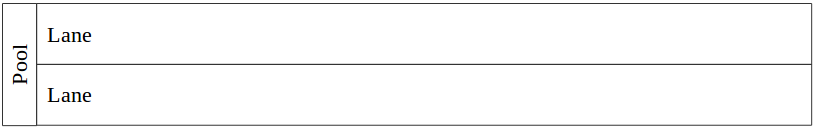
\includegraphics[width=0.8\textwidth]{images/bpmn-pool-swimlanes.png}
	\caption{Pool and Swimlanes}
	\label{fig:recherche:bpmn:poolswimlanes}
\end{figure}
Ein Pool kennzeichnet einen Participant, einen Benutzer oder Benutzerrolle in einem Prozess. Swimlanes ziehen sich über den gesamten Pool und werden dazu benutzt diesen weiter zu unterteilen.

\begin{figure}[H]
	\centering
	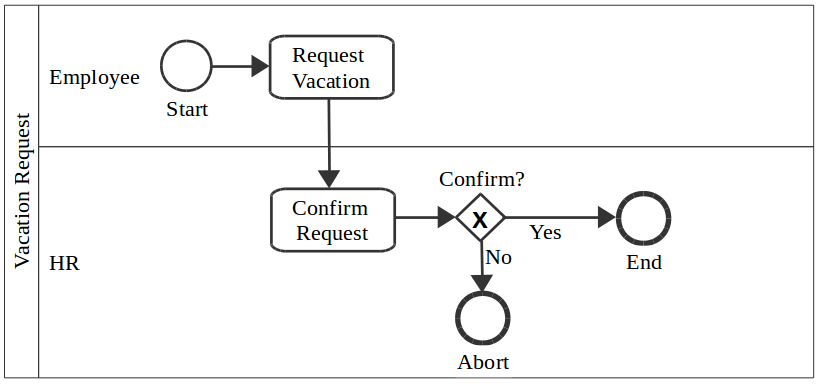
\includegraphics[width=0.8\textwidth]{images/bpmn-example.png}
	\caption{Example}
	\label{fig:recherche:bpmn:example}
\end{figure}
Dies ist eine einfaches Beispiel eines Vacation Request Prozesses. Der Arbeitnehmer startet den Prozess und stellt seine Ferienanfrage. Die Anfrage wird von der Personalabteilung weiterverwendet und entscheidet, ob die Anfrage genehmigt wird oder nicht.

\section{Rahmenbedingungen}
Zu den Rahmenbedingungen gehört die Infrastruktur der travel.ch Webseite, das Entwicklungssystem des Programmierers sowie die etablierten Prozesse der travelwindow AG, welche die Webseite travel.ch betreibt.

\subsection{Travelwindow AG Prozesse}
\label{sec:Recherche:rahmenbedingungen:prozesse}
Die Travelwindow AG ist der Betreiber der Seite travel.ch, auf welcher verschiedene Produkte gekauft werden können. Flüge, Hotel, Badeferien, Städtereisen sowie Hotel und Flug Kombinationen. Da der Buchungsprozess für Hotel und Flug Kombinationen der längste ist, wurde entschieden dass dieser in dieser Arbeit modelliert werden soll. 

\begin{figure}[H]
	\centering
	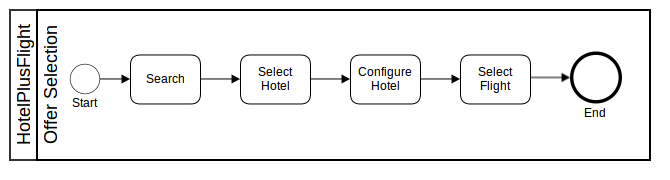
\includegraphics[width=0.8\textwidth]{images/hotelplusflight.png}
	\caption{Hotel plus Flight BPMN Model}
	\label{fig:recherche:rahmenbedingungen:hotelplusflight}
\end{figure}
Der Prozess der Hotel und Flug Suche auf der travel.ch Webseite ist linear. Nach einer Produktsuche muss der Kunde ein Hotel wählen, welches er danach noch weiter Konfigurieren kann. Dabei kann er andere Zimmer- und Verpflegungstypen wählen. Zum Schluss erhält er eine Auswahl von Flügen bevor der Prozess mit einem End Event terminiert.

\subsection{Travelwindow AG API}
\label{sec:Recherche:rahmenbedingungen:api}
Travel.ch besteht aus einer Webseite und einer \Gls{glos:api}. Für die Ausführung der Prozesse via BPMN muss die API angesprochen werden. Diese liefert daten in \Gls{glos:json} aus. Programme für das ausführen des travel.ch BPMN Prozesses muss demnach den Austausch von Daten über eine \Gls{glos:api} mittels \Gls{glos:json} ermöglichen.

\subsection{Betriebsystem}
Die travel.ch Webseite wird über eine \Gls{glos:api} betrieben, welche mittels eines BPMN Programmes abgefragt werden soll. Diese \Gls{glos:api} ist nur vom Firmennetzwerk aus erreichbar. In der Firma sind nur Rechner mit dem Windows Betriebsystem im Einsatz.

Das Entwicklungssystem des Programmierers ist eine Linux Mint Computer. Dabei handelt es sich um ein Unix basiertes Betriebsystem.

Es ist demnach zwingend Notwendig, dass das BPMN Programm auf Windows, sowie auf Unix basierten Betriebssystemen läuft.

\section{Programme}
In diesem Abschnitt werden verschiedene Programme vorgestellt und analysierten, ob sie für die Umsetzung dieses Projekte in Frage kommen. Dazu wird zuvor definiert, was die Anforderungen an das Programm sind.

\subsection{Anforderungen}
In den Abschnitten \cref{sec:Recherche:rahmenbedingungen:prozesse} \nameref{sec:Recherche:rahmenbedingungen:prozesse} und \cref{sec:Recherche:rahmenbedingungen:api} \nameref{sec:Recherche:rahmenbedingungen:api} wurde beschrieben, dass das Programm auf den Betriebsystemen Windows und Unix lauffähig sein muss, sowie die Unterstützung von \Gls{glos:json} basierten \Glspl{glos:api} beinhalten muss.

Gemäss Aufgabenstellung muss das Tool auch die Datentransformation mittels XSLT unterstützen.

\subsection{Programmanalyse}
Activity
Jbpm
Imix
Camuda
Drools (arbeitet mit jbpm)